\subsection{MetaClust}
By clicking on the Toolset tab and then choose MetaClust,
users are directed to MetaClust home page as in Figure~\ref{fig:metaClustHome}.
MetaClust \citep{huo2016meta} aims to perform sample clustering analysis combining multiple transcriptomic studies.
By integrating information from multiple studies of similar biological purposes,
MetaClust can identify an unified intrinsic gene set among all studies, perform weighted clustering analysis using the common intrinsic gene set and
match the clustering patterns across studies to define disease subtypes/cluster types.
The resulting clustering from meta-analysis is more robust and accurate than single study analysis.
The R package for MetaClust module can be found at \url{https://github.com/metaOmics/MetaSparseKmeans}.


\begin{figure}[H]
\begin{center}
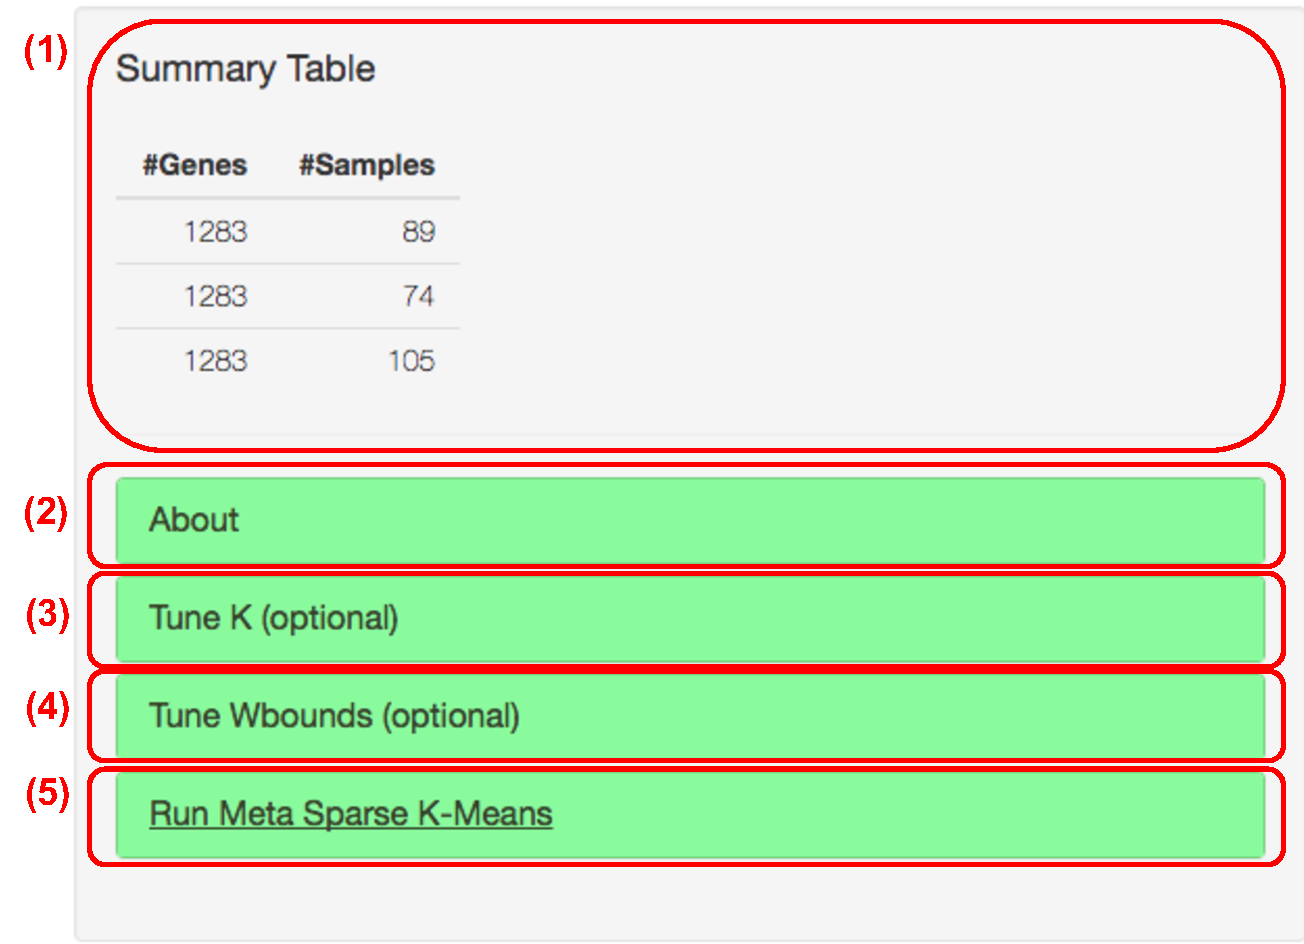
\includegraphics[scale=0.4]{./figure/metaClust/metaClustHome.pdf}
\caption{MetaClust home page}
\label{fig:metaClustHome}
\end{center}
\end{figure}

\subsubsection{Procedure}

Figure~\ref{fig:metaClustHome} shows the home page of MetaClust.
On the top left panel users can see the data summary Table {\color{red} (1)}.
Below there are four tabs. 
About tab {\color{red} (2)} which includes basic introduction of MetaClust, Two tabs for Tune K as well as Wbounds, and the Run Meta Sparse K-Means tab.
Starting with multiple studies, 
we could run MetaSparseKmeans {\color{red} (5)} with pre-specified number of clusters ($K$) and gene selection tuning parameter (Wbounds).
If you are not sure about what are good $K$ and Wbounds, please try Tune $K$ {\color{red} (3)} and Tune Wbounds {\color{red} (4)} panel.

\begin{steps}

\item \textbf{Tune $K$:} 

\begin{figure}[H]
\begin{center}
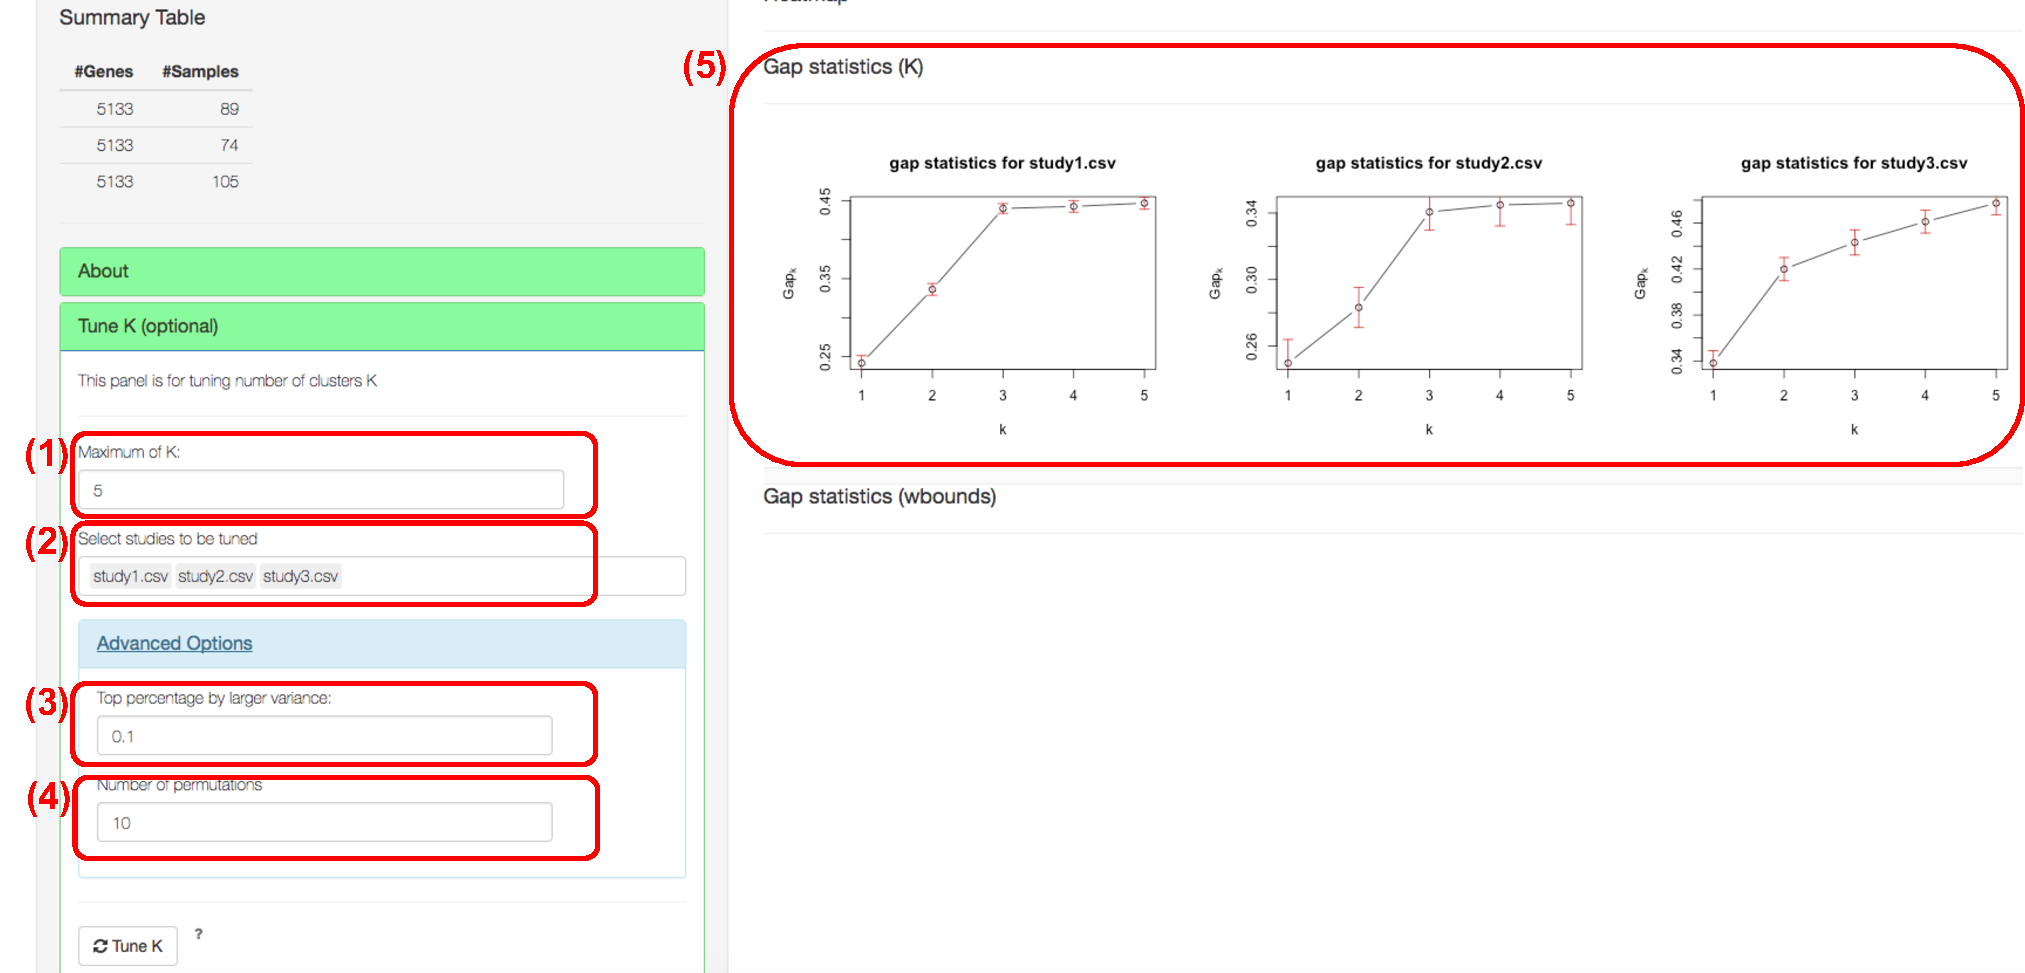
\includegraphics[scale=0.5]{./figure/metaClust/tuneK.pdf}
\caption{Tuning parameter selection for number of clusters}
\label{fig:metaClusttuneK}
\end{center}
\end{figure}

If the users are not sure what is the number of clusters,
they can start to use the Tune $K$ panel as in Figure~\ref{fig:metaClusttuneK}.
Gap statistics will be used to get optimal $K$ for each individual study.
Users need to specify maximum number of $K$ {\color{red} (1)}, which the algorithm will search number of studies from 1 to $K$.
Studies to be tuned can be selected {\color{red} (4)}.
In advanced options, users can further specify number of top variance genes to be included and number of permutations.
But if users don't know the algorithm, please leave them as default.
Top percentage p\% by larger variance means that we will use top p\% larger variance genes to perform gap statistics {\color{red} (3)}.
Number of permutation is the number of bootstrap samples for gap statistics {\color{red} (4)}.
At least 50 bootstrap samples are suggested for a stable result of number of clusters.
By clicking button ``Tune $K$",
we will obtain gap statistics as in Figure~\ref{fig:metaClusttuneK}.
A good $K$ is selected such that the $\mbox{Gap}_k$ is maximized or stabilized across all studies.
From the figure, $K=3$ is preferred since the gap statistics from all three studies become flat {\color{red} (5)}.

\item \textbf{Tune Wbounds:} 

Wbounds directly control number of features selected by metaClust.
If the users are not sure what is a good Wbound,
they can start to use the Tune Wbounds panel as in Figure~\ref{fig:metaClusttuneW}.
\begin{figure}[H]
\begin{center}
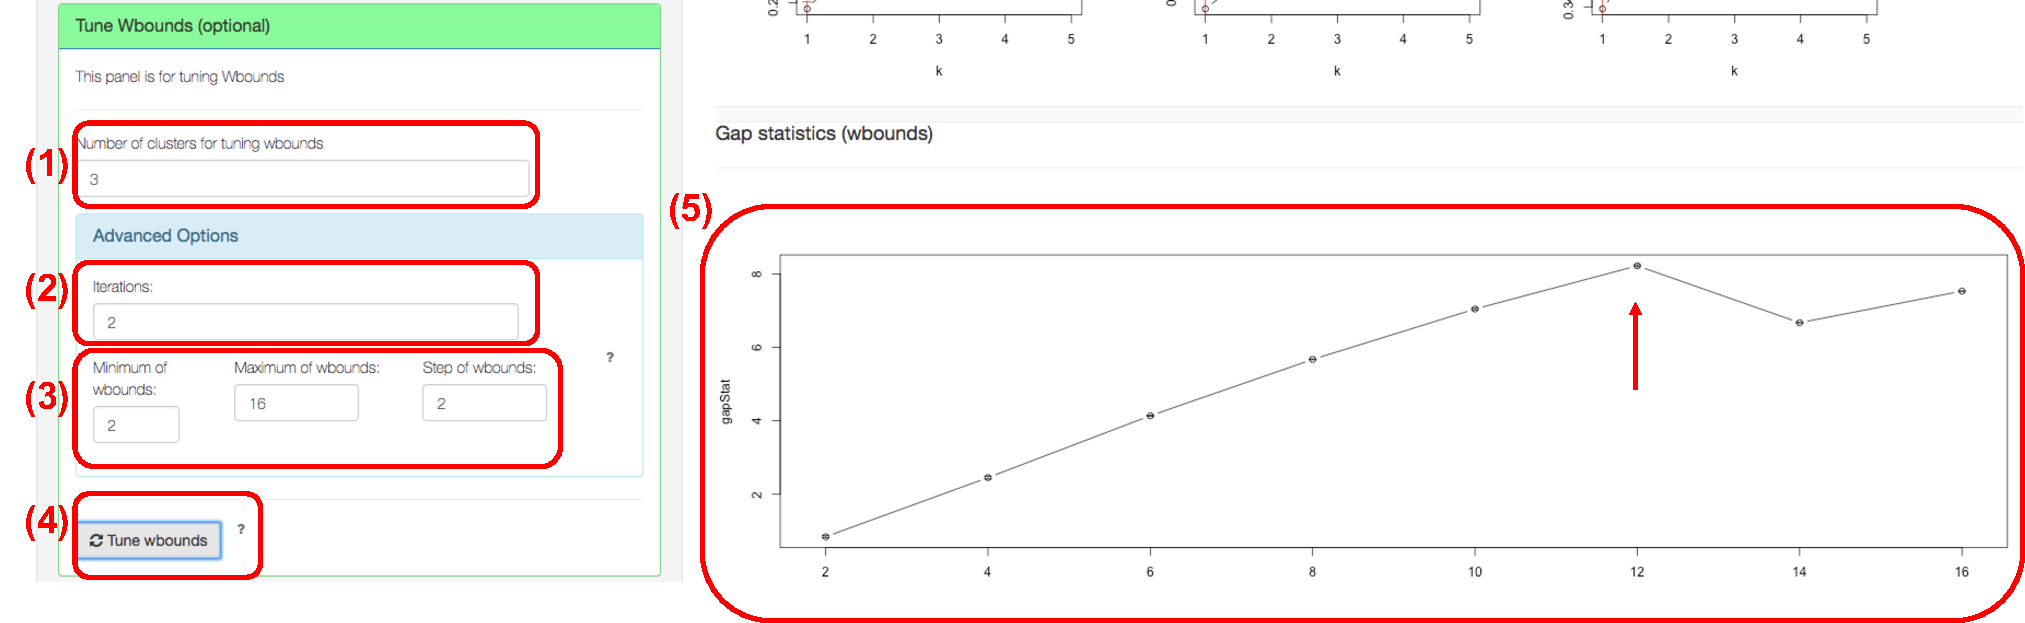
\includegraphics[scale=0.5]{./figure/metaClust/tuneW.pdf}
\caption{Wbound selection}
\label{fig:metaClusttuneW}
\end{center}
\end{figure}
Again,
gap statistics will be used for tuning Wbounds.
Users will specify number of clusters for tuning Wbounds {\color{red} (1)}, which could be obtained from the previous step.
In advanced options, users can further specify the number of iterations and the range of candidate Wbounds.
But if users don't know the algorithm, please leave them as default.
Iterations {\color{red} (2)} specify number of bootstrap samples for gap statistics.
Users also need to specify the searching space of Wbounds by minimum of Wbounds, maximum of Wbounds and Step of Wbounds {\color{red} (3)}.
After all these steps are set,
user can click on ``Tune Wbounds" button {\color{red} (4)}.
The results will be shown in Figure~\ref{fig:metaClusttuneW} {\color{red} (5)}.
Wbound=12 is preferred since the corresponding gap statistics is maximized (where the red arrow indicates).

\item \textbf{Run MetaClust:} 

Under Run Meta Sparse K-Means panel,
user can specify the number of clusters {\color{red} (1)}, Wbounds {\color{red} (2)} and run MetaClust {\color{red} (5)} 
as in Figure~\ref{fig:mskmRes}.
\begin{figure}[H]
\begin{center}
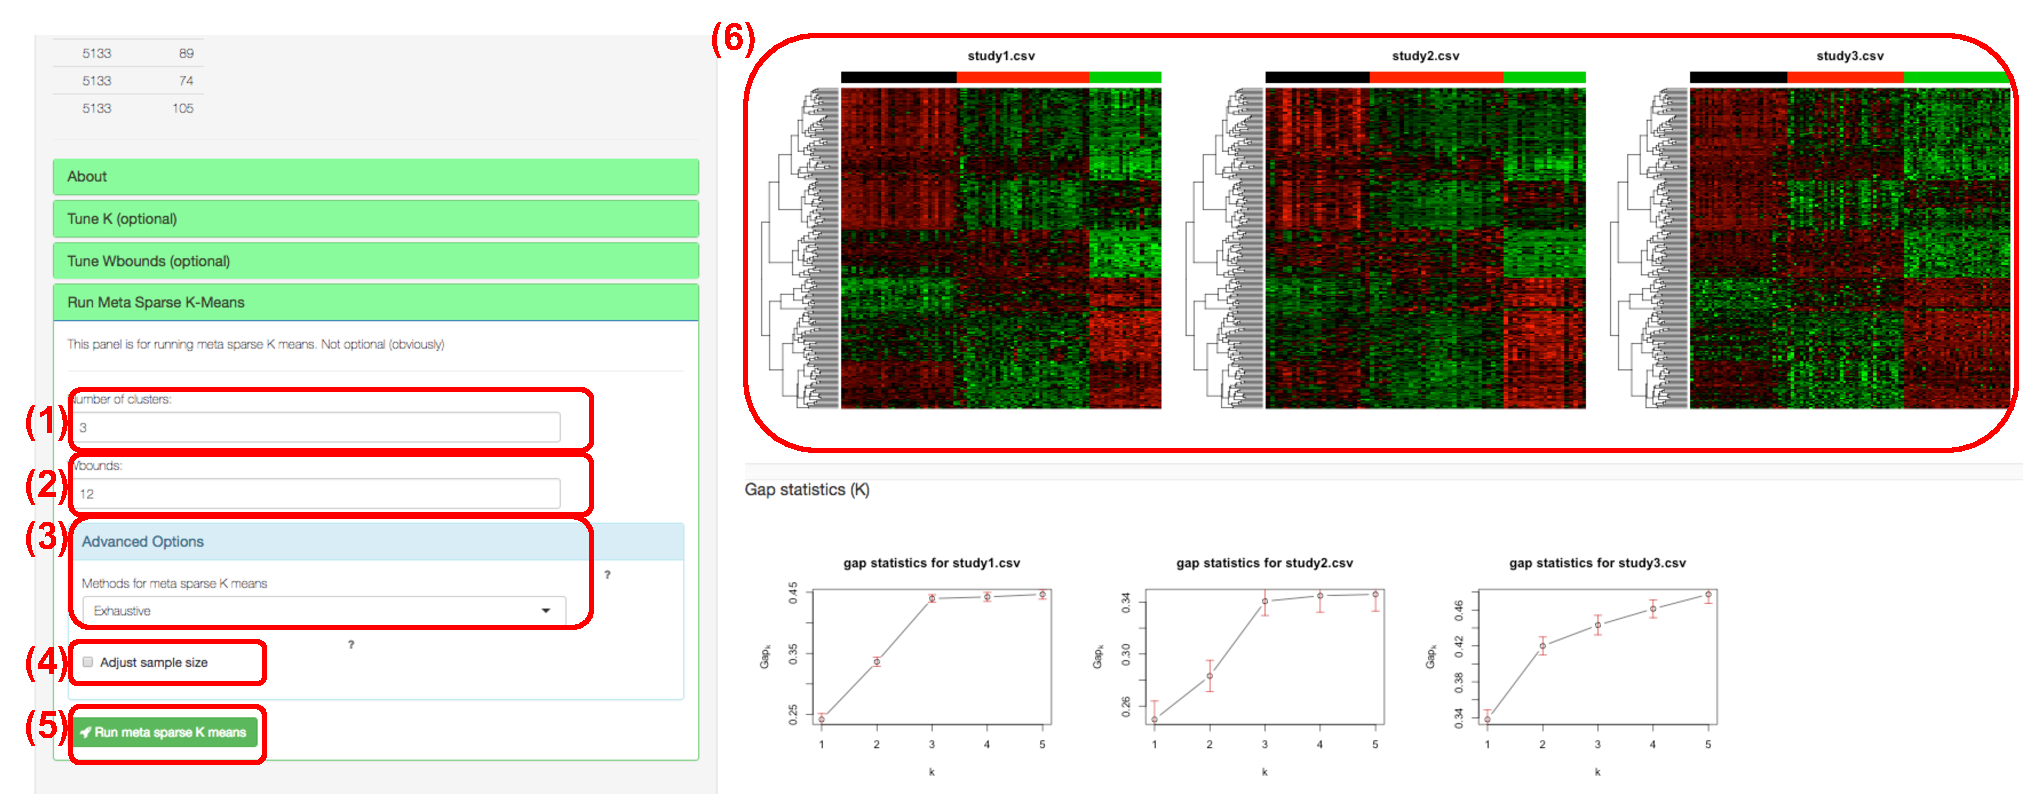
\includegraphics[scale=0.5]{./figure/metaClust/mskmRes.pdf}
\caption{Result for MetaClust}
\label{fig:mskmRes}
\end{center}
\end{figure}
In advanced options (for which users are not suggested to change if they are not familiar with the algorithm), 
There are three clustering matching methods {\color{red} (3)}: Exhaustive, linear, MCMC.
Exhaustive is suggested if the data is not large.
Linear will perform smart search and get solution much faster than Exhaustive, 
but it may yield less accurate results with very low probability.
MCMC is suitable if many studies and clusters are provided.
Adjust sample size checkbox (at position {\color{red} (5)}) allows users to adjust sample size effect.
After number of clusters and Wbounds are specified,
users can click on Run meta sparse $K$ means and obtain results as Figure~\ref{fig:mskmRes}.

\end{steps}

\textbf{Complete List of Options:} 
\begin{enumerate}
\item Tune $K$ (** optional)
\begin{itemize}
\item Maximum of $K$: the maximum number of $K$ that gap statistics will step through.
\item Top percentage by larger variance: Top percentage p\% by larger variance means that we will use top p\% larger variance genes to perform gap statistics.
\item Number of permutaitons: Number of permutation is number of bootstrap samples for gap statistics.
\item Select studies to be tuned: Studies to be tuned.
\item Tune $K$: start tuning $K$.
\end{itemize}
\item Tune Wbounds (** optional)
\begin{itemize}
\item Number of clusters for tuning wbounds: number of clusters for tuning Wbounds.
\item Iterations: Iterations are number of bootstrap samples for gap statistics.
\item Minimum of wbounds: lower bound of the searching space of Wbounds.
\item Maximum of wbounds: upper bound of the searching space of Wbounds.
\item Step of of wbounds: stepsize of the searching space of Wbounds.
\item Tune wbounds: start tuning wbounds.
\end{itemize}
\item Run Meta Sparse $K$-means: 
\begin{itemize}
\item Number of clusters: number of clusters. Can be tuned from Tune $K$ option.
\item Wbounds: control numbers of selected features. Can be tuned from Tune Wbounds option.
\item Methods for MetaClust: Exhaustive is suggested if the data is not large.
Linear will perform smart search and get solution much faster than Exhaustive, 
but it may yield less accuracy.
MCMC might by very time consuming.
\item Adjust sample size: adjust sample size effect.
\item Run meta sparse Kmeans: start tuning wbounds.
\end{itemize}

\end{enumerate}


\subsubsection{Results}

We used the leukemia data to demonstrate the MetaClust module.
After merging the three datasets, we didn't filter out any genes (filter 0\% genes by mean and 0\% by variance) thus 5133 genes remained.
Detailed descriptions of these studies can be found in Table~\ref{tab:realDataLeukemia}. 
In this example, we do not need the extra label information.
The result is shown in Figure~\ref{fig:mskmRes} {\color{red} (5)}.
We obtained unified feature selection across all studies.
The clusters are well separated in each study and the cluster patterns are consistent across all studies.
The clustering heatmaps and labels are saved in the MetaClust folder.










